The Jeffery Orbits describe the motion of an ellipsoidal particle in stokes shear flow as a function of time. The inital orbits found by Jeffery were for axis-symmetrical ellipsoidal particles, but was generalized by Yarin et al \cite{Yarin} to triaxial particles. Note that Jeffery Orbits sometimes refers only to the symmetric orbits but I will in this thesis refer to the generalized orbits as the Jeffrey Orbits. The generalized equations of motion found by Yarin et al was

\begin{subequations}\label{eq:jeffrey}
\begin{align}
\frac{d\theta}{dt} 	&= (g_2 \sin \psi + g_3 \cos \psi ) \sin \theta \\
\frac{d\phi}{dt} 	&= \tfrac{1}{2} + g_3\sin \psi - g_2 \cos \psi\\
\frac{d\psi}{dt}	&= g_1 + (g_2\cos \psi - g_3\sin \psi) \cos \theta \\
\end{align}
\end{subequations}

where the functions  $g_i$ are defined as

\begin{subequations}
\begin{align}
g_1 &= \frac{a_y^2 - a_z^2}{2(a_y^2 + a_z^2)} 
		\left(-\tfrac{1}{2}(\cos^2 \theta + 1 )\sin 2\phi \sin 2\psi + \cos\theta \cos 2\phi \cos 2\psi \right), \\
g_2 &= \frac{a_z^2 - a_x^2}{2(a_x^2 + a_z^2)}
		\left( -\cos\theta \sin 2\phi \sin\psi  +  \cos 2\phi \cos\psi \right), \\
g_3 &= \frac{a_x^2 - a_y^2}{2(a_x^2 + a_y^2)}
		\left( \cos\theta \sin 2\phi \cos\psi + \cos 2\phi \sin\psi \right)
\end{align}
\end{subequations}

where the angles are defined as can be seen in figure \ref{fig:eulerangles}. We can make a few key observations 

Solutions to the equations of motions can be found with numerical methods as shown by CITE SOME DUDE but one has to be careful to convert to the right coordinates. 

The orbits for different initial conditions can be plotted in a Poincaré map, also known as a Surface of Section (S.O.S) \cite{poincare} for $\phi = 0$. A few such maps can be seen in figure \ref{fig:poincaremaps}. A simplified explanation of the Poincare map is that a particle starting on some point on a line in the map will follow along that line the next time it intersects with the section, in our case when the particle has $\phi=0$. 

For a particle with a small asymmetry there are essentially three classes of orbits.

\begin{enumerate}
\item Periodic. For larger $\left|\theta\right|$ there is little variation and the particle is largely periodic with fluctuations too small to measure.
\item Quasi-periodic bent: For intermediate $\left|\theta\right|$ the amplitude of $\cos(\theta)$ changes noticeably but does not change sign.
\item Quasi-periodic circular: For small $\left|\theta\right|$ the amplitude of $\cos(\theta)$ will change noticeably and change sign from positive to negative.
\end{enumerate}

These three different types of orbits are illustrated in \ref{fig:orbittypes} and also shows .

\begin{figure}[H]
\centering
\begin{subfigure}[3a]{0.40\textwidth}
\includegraphics[width=\textwidth]{figures/theory/map.pdf}
\caption{A poincare map}\label{fig:orbitmap}
\end{subfigure}\hspace{1em}%
\begin{subfigure}[3b]{0.40\textwidth}
\includegraphics[width=\textwidth]{figures/theory/orbit.pdf}
\caption{The time series for the components \\ of the unit vector.}\label{fig:orbitparams}
\end{subfigure}
\caption{A poincare map and three orbits for the Jeffery orbits of a particle with $\lambda=7$ and $\epsilon=0.05$. The three orbits highlight the three different kinds of orbit, the quasi periodic circular orbit in blue, the quasi-periodic bent orbit in red and the periodic in green. We see that while $n_x$ and $n_y$}
\label{fig:orbittypes}
\end{figure}

\subsection{Winding Number}
The quasi-periodic orbits are also referred to as double-periodic. This is referring to the fact that the variations that are seen in figure \ref{fig:orbitparams} are periodic as well. The ratio between the two periods is referred to as the winding number $\omega$, or simply
\begin{equation}\label{eq:winding}
\omega = \frac{\theta_1}{\theta_2}.
\end{equation}

which is illustrated in figure \ref{fig:windingDef}.

\begin{figure}[H]
\begin{center}
\includegraphics[width=0.7\textwidth]{figures/theory/WindingNrFixed.pdf}
\end{center}
\caption{The winding number is defined as the quotient between the longer and shorter period. This is the $n_z$ plot bent quasi periodic orbit from figure \ref{fig:orbittypes} highlighting the short period $\theta_2$ which is simply the period of $\phi$ and the longer period $\theta_1$.}
\label{fig:windingDef}
\end{figure}

This can also be thought of as the number of steps travelled on the poincare map before coming back to where it 
started, divided by the number of laps it takes. This number is the same for any point along a given orbit on the 
poincare map but varies greatly for different orbits as well as for different asymmetries. The winding numbers for
 orbits a slice along $\psi=0$ for $\epsilon=\{0.01, 0.05, 0.10\}$ can be seen in figure \ref{fig:windingdifferent}
 
\begin{figure}[H]
\begin{center}
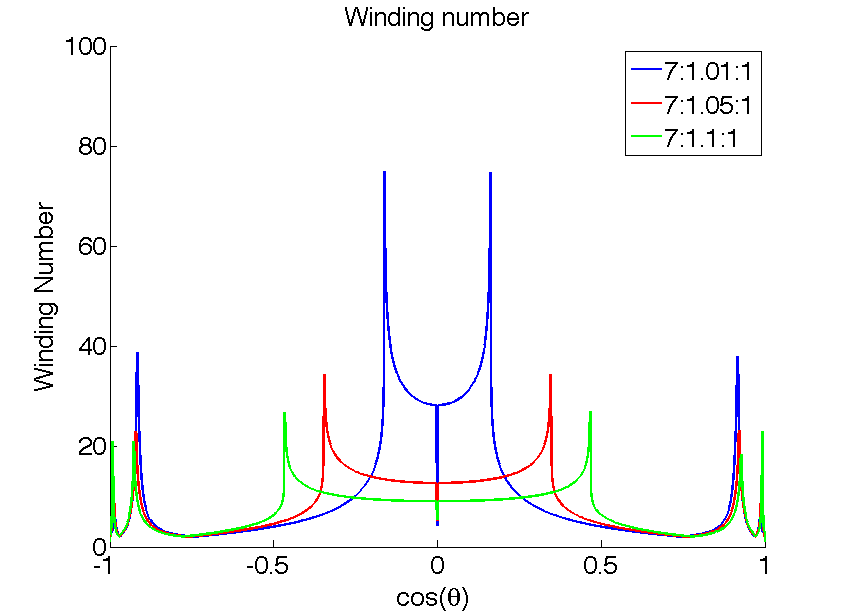
\includegraphics[width=0.7\textwidth]{figures/theory/WindingTrend.png}
\end{center}
\caption{The winding number as a function of $\cos(\theta)$ for three different asymmetries. The sharp edge that occurs centered around zero is when the circular orbits break into bent orbits as mentioned previously. We see that a lower asymmetry leads to a sharper difference between the circular and the bent orbits.}
\label{fig:windingdifferent}
\end{figure}
